\documentclass{article}
\usepackage{graphicx}
\usepackage{amsmath}
\usepackage{footnote}
\usepackage{hyperref}

\title{The Relationship Between Rainfall and Mushroom Growth Rate}
\author{Tianning Zhu}
\date{\ 27 Oct 2024}

\begin{document}

\maketitle

\section*{Abstract}
This report investigates the relationship between rainfall and mushroom growth rate using a synthetic dataset. A linear regression analysis was conducted to determine the strength and nature of this relationship. The results indicate a significant correlation, suggesting that rainfall may influence mushroom growth.

\section*{Introduction}
It has been shown that there is a correlation between rainfall and mushroom growth rate. However, it is unclear whether this holds for every possible dataset and whether the relation is linear on the original scale. Thus, the research question is: Is there a relation between rainfall and mushroom growth rate on the logarithmic scale?

\section*{Background}
Previous studies have indicated that environmental factors, including rainfall, significantly affect mushroom growth. For instance, a study by C. J. Krebs et al. (2008) demonstrated that increased precipitation correlates with higher yields of various mushroom species. This suggests that understanding the relationship between rainfall and mushroom growth could be crucial for agricultural practices.

\section*{Data and Method}
The dataset used for this analysis is titled \texttt{rain\_mushrooms\_with\_high\_noise.csv}, which contains synthetic data on rainfall (in mm) and mushroom growth rate (in grams). A linear regression analysis was performed to assess the relationship between these two variables. The analysis was conducted using Python, employing libraries such as Pandas, NumPy, and SciPy.

\section*{Results}
The linear regression analysis yielded the following results:
\begin{itemize}
    \item Slope: 5.7726
    \item Intercept: -216.4093
    \item R-squared: 0.8965
    \item P-value: 4.5356e-50
    \item Standard Error: 0.1981
\end{itemize}
The R-squared value indicates that approximately 89.65\% of the variance in mushroom growth rate can be explained by rainfall. The p-value suggests that the relationship is statistically significant.

\begin{figure}[h]
    \centering
    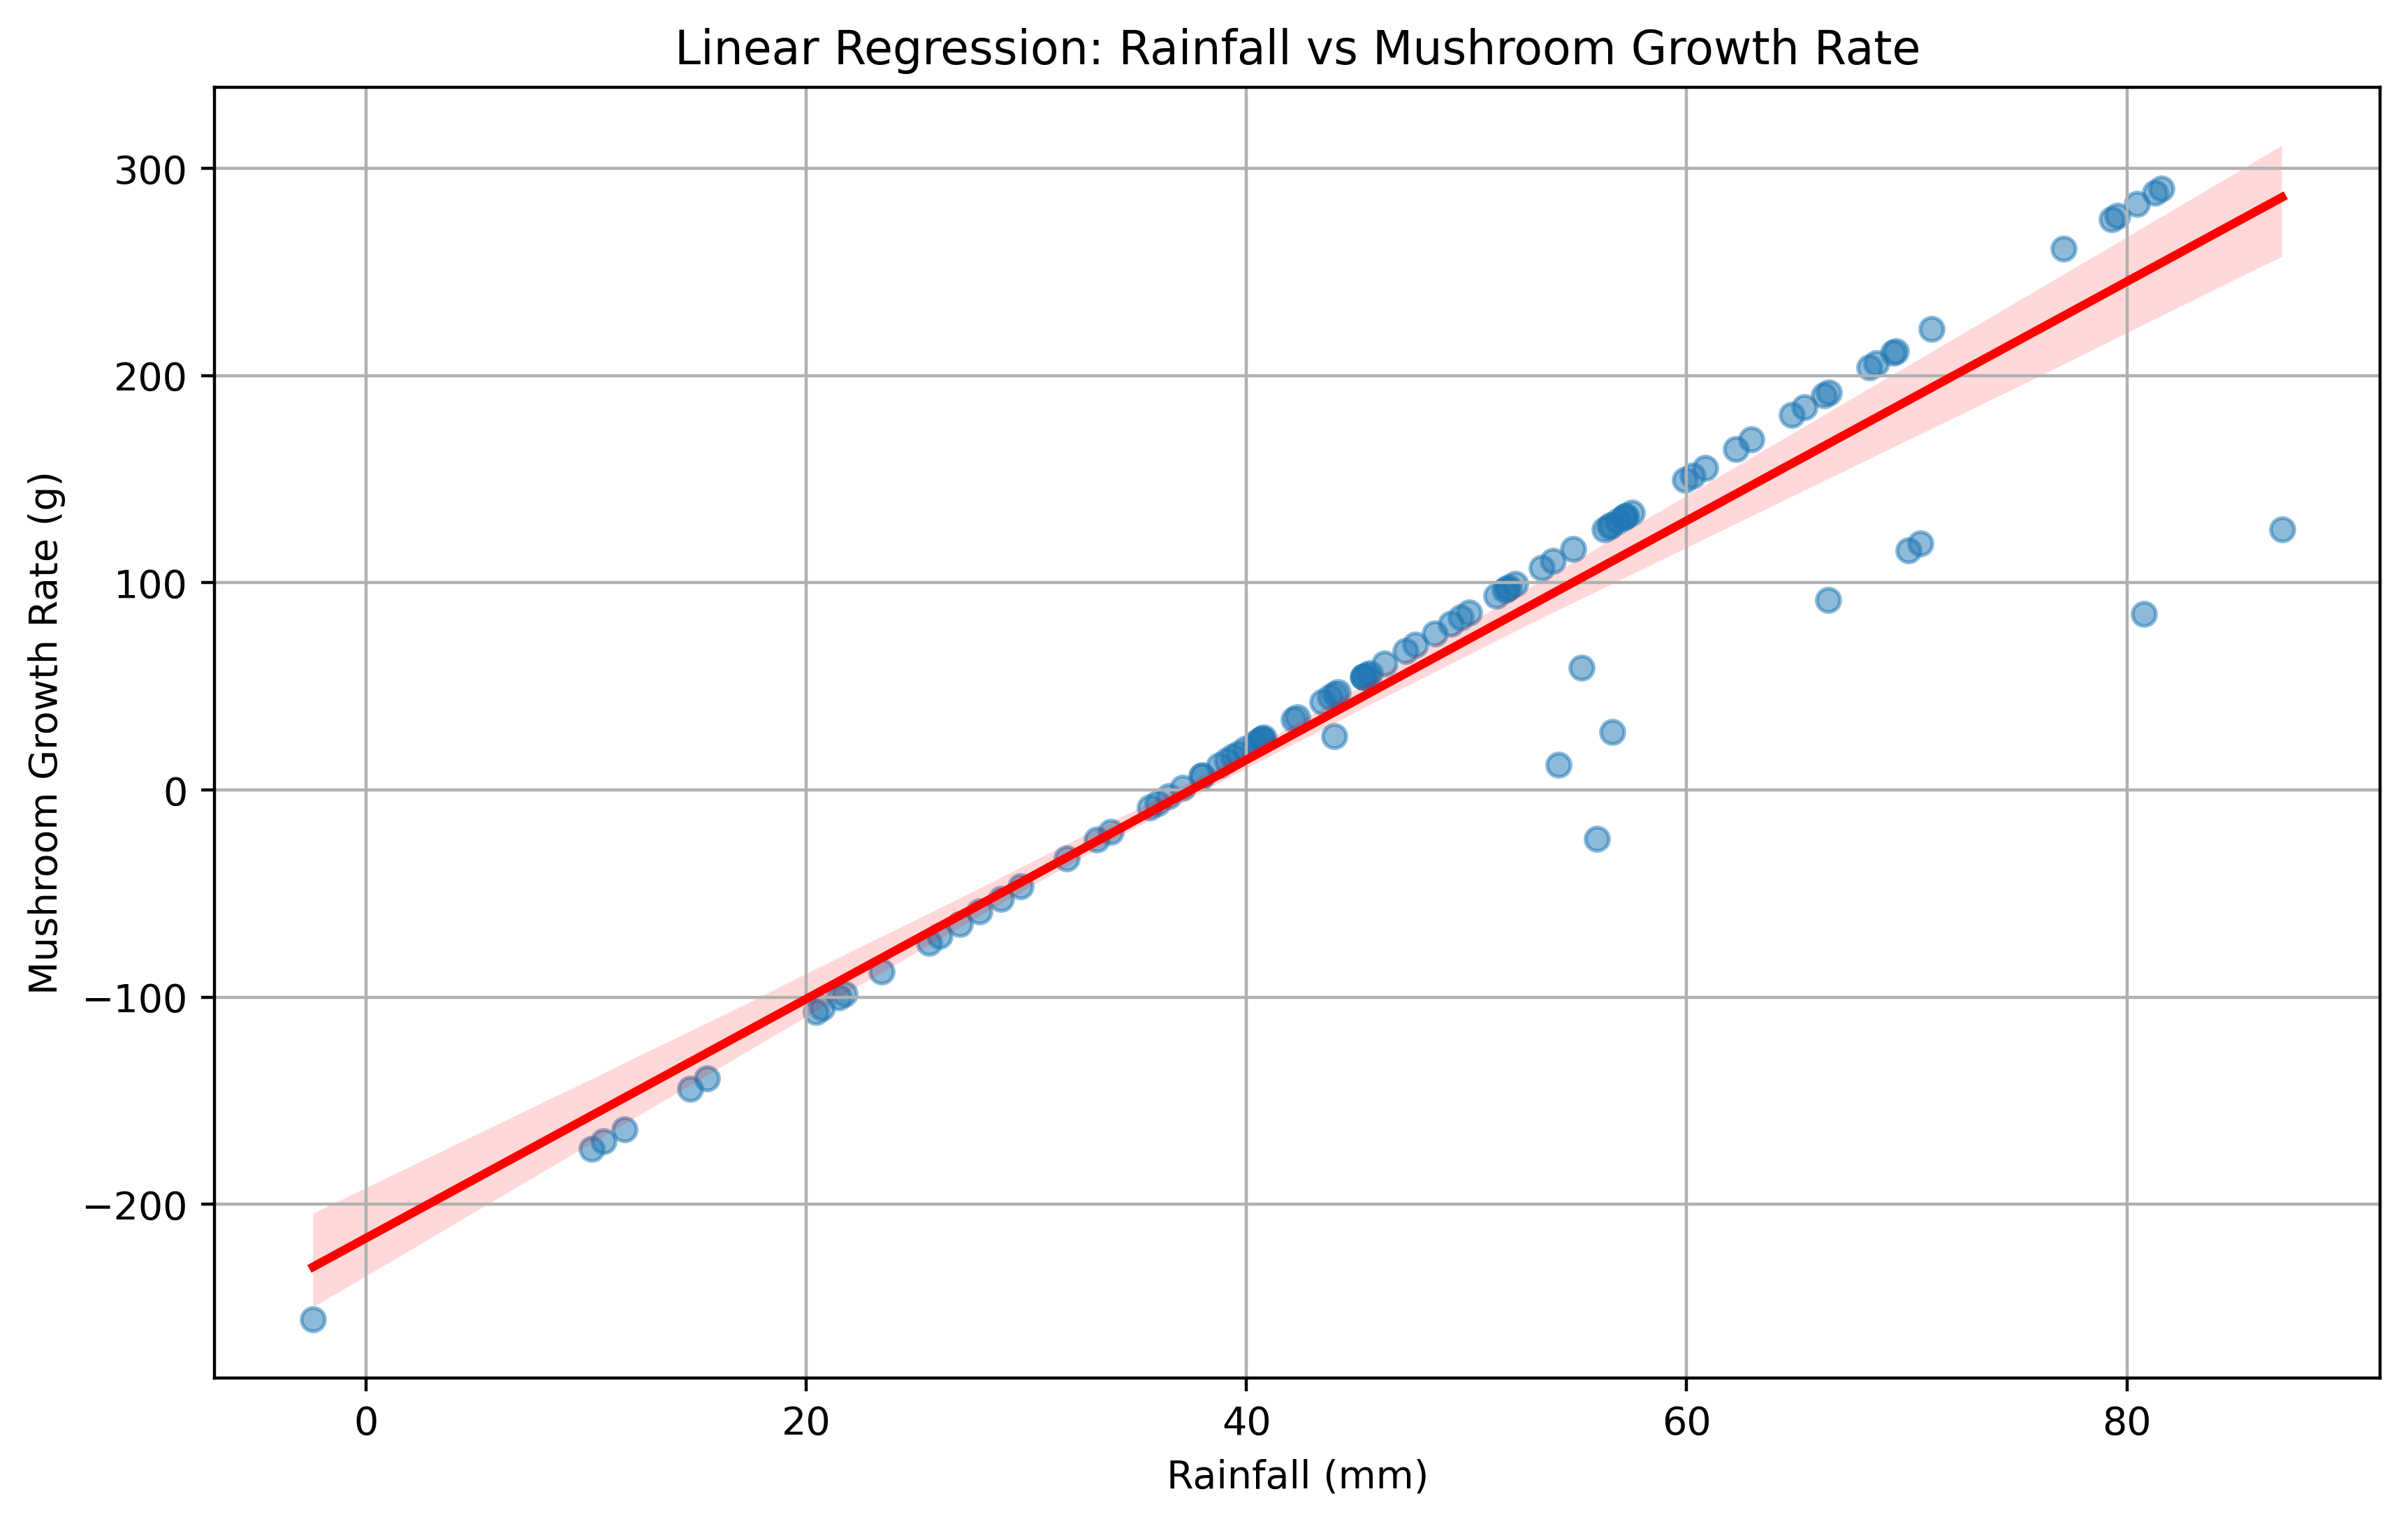
\includegraphics[width=0.8\textwidth]{adjusted_fake_rain_mushrooms_with_high_noise.png}
    \caption{Linear Regression: Rainfall vs Mushroom Growth Rate}
    \label{fig:regression}
\end{figure}

\section*{Discussion}
The results indicate a strong positive relationship between rainfall and mushroom growth rate. The slope of the regression line suggests that for each additional millimeter of rainfall, the growth rate of mushrooms increases by approximately 5.77 grams. This finding has implications for agricultural practices, particularly in regions where mushroom cultivation is significant.

\section*{Conclusion}
In summary, the analysis demonstrates a significant linear relationship between rainfall and mushroom growth rate, highlighting the importance of rainfall in mushroom cultivation.

\section*{References}
C. J. Krebs, Patrick Carrier, S. Boutin, R. Boonstra, and Elizabeth Hofer. (2008). Mushroom crops in relation to weather in the southwestern Yukon. \textit{Botany}
 
\end{document}
